\question{10.1}{
    Bij een onderzoek naar de rookgewoonten van Nederlanders van $18$ jaar en ouder werden door loting $200$ proefpersonen gekozen die vervolgens werden ingedeeld naar leeftijd en naar rookgewoonte.
    De resultaten waren als volgt:
    \begin{center}
        \renewcommand{\arraystretch}{1.25}
        \begin{tabular}{ccccc}
            \toprule
                \multicolumn{5}{c}{{\bfseries Leeftijd}} \\
            \cmidrule{1-1} \cmidrule{2-2} \cmidrule{3-3} \cmidrule{4-4} \cmidrule{5-5}
                & $\mathbf{18-<30}$ & $\mathbf{30-<45}$ & $\mathbf{45}$ \textbf{en ouder} & {\bfseries Totaal} \\
            \cmidrule{1-1} \cmidrule{2-2} \cmidrule{3-3} \cmidrule{4-4} \cmidrule{5-5}
                Roker & $25$ & $35$ & $20$ & $80$ \\
                Niet-roker & $55$ & $25$ & $40$ & $120$ \\
            \cmidrule{1-1} \cmidrule{2-2} \cmidrule{3-3} \cmidrule{4-4} \cmidrule{5-5}
                Totaal & $80$ & $60$ & $60$ & $200$ \\
            \bottomrule
        \end{tabular}
    \end{center}
    We gaan met behulp van de chikwadraattoets onderzoeken of de indelingen naar leeftijd en rookgewoonte al dan niet afhankelijk van elkaar zijn.
    We toetsen met $\alpha=0,01$.
    De nulhypothese luidt: $H_0:$ onafhankelijkheid.
}
\begin{enumerate}[label=(\alph*)]
    \item Bereken de \emph{expected}-tabel.
    \answer{
        Om de \emph{expected}-tabel te bepalen, starten we vanuit een lege tabel waarin alleen de totalen (van de rijen en kolommen respectievelijk) gegeven zijn:
        \begin{center}
            \renewcommand{\arraystretch}{1.25}
            \begin{tabular}{ccccc}
                \toprule
                    \multicolumn{5}{c}{{\bfseries Leeftijd}} \\
                \cmidrule{1-1} \cmidrule{2-2} \cmidrule{3-3} \cmidrule{4-4} \cmidrule{5-5}
                    & $\mathbf{18-<30}$ & $\mathbf{30-<45}$ & $\mathbf{45}$ \textbf{en ouder} & {\bfseries Totaal} \\
                \cmidrule{1-1} \cmidrule{2-2} \cmidrule{3-3} \cmidrule{4-4} \cmidrule{5-5}
                    Roker & $$ & $$ & $$ & $80$ \\
                    Niet-roker & $$ & $$ & $$ & $120$ \\
                \cmidrule{1-1} \cmidrule{2-2} \cmidrule{3-3} \cmidrule{4-4} \cmidrule{5-5}
                    Totaal & $80$ & $60$ & $60$ & $200$ \\
                \bottomrule
            \end{tabular}
        \end{center}

        Voor iedere cel in de tabel bepalen we de expected frequentie met de formule:
        \[
            E_{ij} = \frac{\text{rijtotaal}_{i} \cdot \text{kolomtotaal}_{j}}{\text{totaal}}
        \]

        Dit geeft de volgende \emph{expected}-tabel:
        \begin{center}
            \renewcommand{\arraystretch}{1.25}
            \begin{tabular}{ccccc}
                \toprule
                    \multicolumn{5}{c}{{\bfseries Leeftijd}} \\
                \cmidrule{1-1} \cmidrule{2-2} \cmidrule{3-3} \cmidrule{4-4} \cmidrule{5-5}
                    & $\mathbf{18-<30}$ & $\mathbf{30-<45}$ & $\mathbf{45}$ \textbf{en ouder} & {\bfseries Totaal} \\
                \cmidrule{1-1} \cmidrule{2-2} \cmidrule{3-3} \cmidrule{4-4} \cmidrule{5-5}
                    Roker & $\frac{80 \cdot 80}{200}=32$ & $\frac{80 \cdot 60}{200}=24$ & $\frac{80 \cdot 60}{200}=24$ & $80$ \\
                    Niet-roker & $\frac{120 \cdot 80}{200} = 48$ & $\frac{120 \cdot 60}{200} = 36$ & $\frac{120 \cdot 60}{200} = 36$ & $120$ \\
                \cmidrule{1-1} \cmidrule{2-2} \cmidrule{3-3} \cmidrule{4-4} \cmidrule{5-5}
                    Totaal & $80$ & $60$ & $60$ & $200$ \\
                \bottomrule
            \end{tabular}
        \end{center}
    }

    \item Bereken de toetsingsgrootheid $\chi^2$.
    \answer{
        De theoretische toetsingsgrootheid $X^2$ bepalen we aan de hand van de volgende formule:
        \begin{align*}
            X^2  &= \sum_{i,j} \frac{(O_{ij} - E_{ij})^2}{E_{ij}},
        \end{align*}
        waarbij $i = 1,2$ de index van de rij is, en $j = 1,2,3$ de index van de kolom is.
        Dit geeft in dit specifieke geval een geobserveerde toetsingsgrootheid 
        \begin{align*}
            \chi^2  &= \sum_{i,j} \frac{(O_{ij} - E_{ij})^2}{E_{ij}} \\
                    &=\frac{(O_{11} - E_{11})^2}{E_{11}} + \frac{(O_{12} - E_{12})^2}{E_{12}} + \ldots + \frac{(O_{23} - E_{23})^2}{E_{23}} \\
                    &= \frac{(25 - 32)^2}{32} + \frac{(35 - 24)^2}{24} + \ldots + \frac{(40 - 36)^2}{36}\\
                    &\approx 12,0660
        \end{align*}
    }

    \item Hoeveel vrijheidsgraden heeft de chikwadraatverdeling die gebruikt moet worden?
    \answer{
        Bij een $\chi^2$-toets voor onafhankelijkheid van twee nominale variabelen is het aantal vrijheidsgraden gelijk aan het aantal cellen waarvoor je een waarde vrij kunt kiezen.
        Dit is gelijk aan 
        \[
            \text{df} = (\#\text{rijen}-1) \cdot (\#\text{kolommen}-1) = (2-1)\cdot(3-1) = 2.
        \]
        In deze hypothesetoets voor onafhankelijkheid heeft de toetsingsgrootheid een chikwadraatverdeling met $\text{df}=2$ vrijheidsgraden.
    }

    \item Geef het kritieke gebied aan van de grootheid $X$.
    \answer{
        Merk op dat onafhankelijkheid waarschijnlijker is als de toetsingsgrootheid dichter bij 0 ligt.
        Dit volgt uit de formule van de toetsingsgrootheid $X$, omdat in dat geval de observed frequenties dicht in de buurt van de expected frequenties liggen.

        Het kritieke gebied is dus van de vorm $[g, \infty)$, waarbij $g$ de grenswaarde is waarvoor geldt $P(X \ge g) = \alpha$.
        Dit kunnen we met de grafische rekenmachine bepalen aan de hand van 
        \begin{align*}
            y_1 &= \chi^2\text{cdf}(\text{lower}=x; \text{upper}=10^{10}; \text{df}=2) \\
            y_2 &= \alpha=0,01
        \end{align*}
    
        De numerieke solver geeft $x \approx 9,2103$.
        Dat betekent dat het kritieke gebied gelijk is aan $[9,2103; \infty)$.

        \begin{center}
            \resizebox{0.9\textwidth}{!}{
                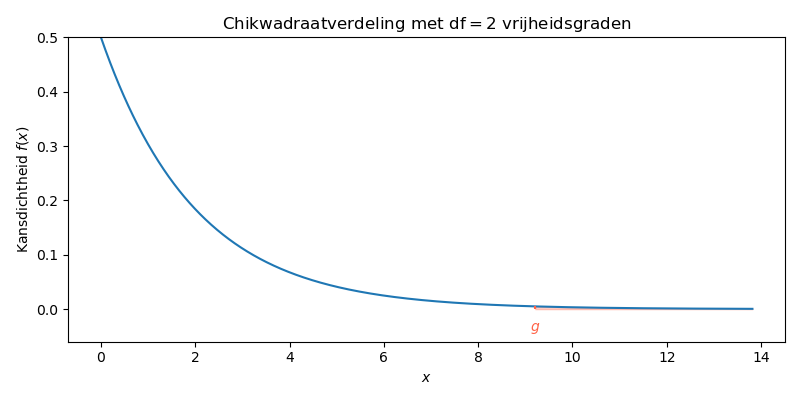
\includegraphics{opg_10.1.png}
            }
        \end{center}
    }

    \item Wat is uw eindconclusie?
    \answer{
        De geobserveerde toetsingsgrootheid $\chi^2 \approx 12,0660$ ligt in het kritieke gebied, omdat $12,0660 > 9,2103$.
        Dit betekent dat de nulhypothese $H_0$ wordt verworpen.
        Er is voldoende bewijs om aan te nemen dat de twee nominale variabelen ``leeftijd'' en ``rookgewoonte'' afhankelijk zijn van elkaar.
    }
\end{enumerate}